\section{The Mathematical Model}
Before discussing the details of our implementation, we would like to introduce the terms and models we used during the project to solve our problem.
We model the image that we are trying to reconstruct as a square grid, $G$, of size $q^2$. Each photon beam is represented as a line passing through this grid. The angle of a particular emission is denoted by $\sigma$ and the number of parallel lines is denoted $n$. Now the $i$'th line for some angle $\sigma'$ can be written as $(\sigma', i)$. Note that the offset between each line must be known. Let this distance be denoted by $\delta$. Since the resolution of the reconstructed image is dictated by $\delta$, we can deduce that the distance between each grid-line in $G$ is also $\delta$. Stated in another way: the size of a pixel in the reconstruction is $\delta^2$. The energy upon exit of each line is stored in a vector of size $m$, denoted $\mathbf{y}$.

For each of the $m$ angles a discretization of the $n$ lines is needed. This is done by dividing each line into the segments between its intersections with the grid. Once these intersections have been obtained, the lengths between each adjacent pair of intersections can be calculated, as they are used to approximate the integral that describes the attenuation along that line. For each line, a matrix with the same size as the grid will be produced. At the general entry $(i,j)$ this matrix has the length of a line segment, if the line passes through the corresponding cell in the grid, otherwise zero. 

This results in a total of $n$ matrixes per emission. Let the collection of these $n$ matrixes form a row in the matrix $\mathbf{A}$, giving a total of $m$ rows. We are now ready to write the actual problem:
$$
  \text{argmin}_{\mathbf{x}} ~~ || \mathbf{Ax} - \mathbf{y} ||^{2}
$$
Here $\mathbf{x}$ denotes the attenuation coefficients, which form the image, and is of length $m$.
While approximating $\mathbf{x}$ is the overarching goal of the tomographic reconstruction, the main task in this project will be to construct the $\mathbf{A}$ matrix in a fast manner.\\

The general situation of a line $(\sigma', i)$ passing through $G$ is shown in figure \ref{fig:intersections}.
% TODO: UPDATE TO REFLECT REFERENCES
\begin{figure}[H]
  \centering
  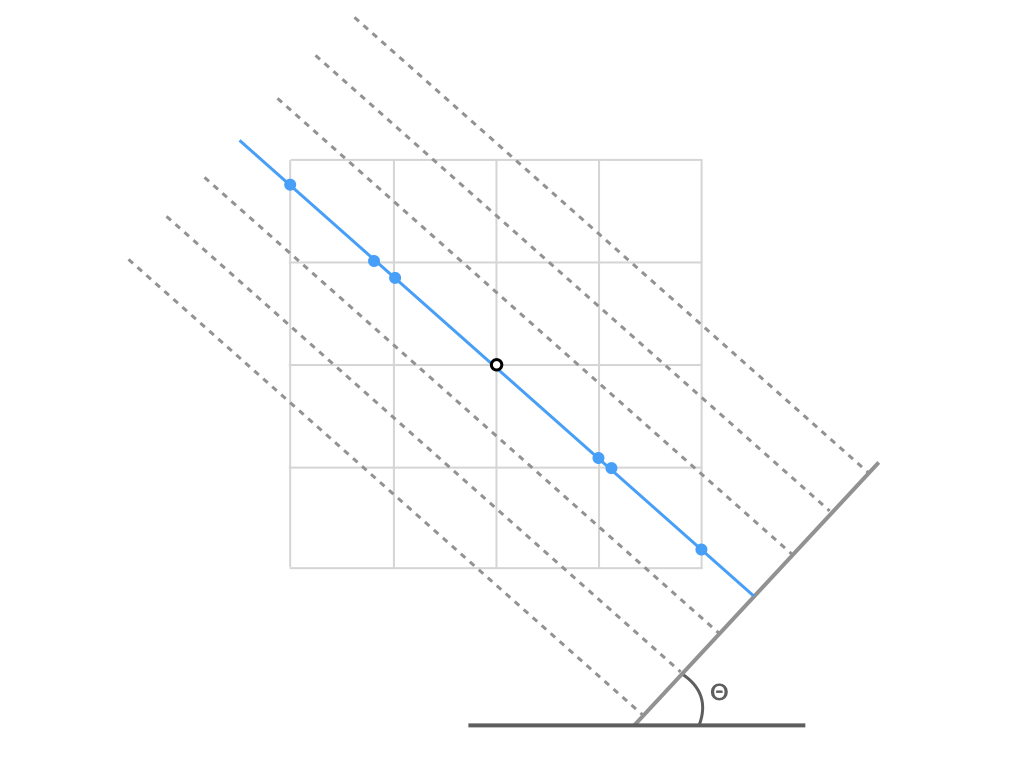
\includegraphics[width=0.9\textwidth]{figures/intersections.png}
  \caption{Grid intersections from ray line}
  \label{fig:intersections}
\end{figure}
$G$ has its origin in the top-left corner. Futhermore the center of $G$ is shown as \texttt{o} in figure \ref{fig:intersections}. Note that each intersection between this line and the grid is a point on the line where either the x or y-component is a whole number. This notion lets us rely on the standard linear equation for lines:
\begin{align}\label{line}
    y = ax + b
\end{align}

We now present equations for computing $a$ and $b$ for a general line. 
\begin{align}
  \label{eq:slope} a &= \tan (\theta + 90) \\[8pt]
  \label{eq:y_intersection} b &= i \cdot \frac{\delta}{\cos (90 - \theta)} + (\texttt{o}_y - a \cdot \texttt{o}_x)
\end{align}
When computing $a$ we add $90$ degrees to $\theta$, to reflect that we are using the angle on the left side of the line, not on the right. For every scan angle, all lines have the same slope, since they are parallel.
The equation for $b$ is a little more complicated, since we wish for the middle line to pass through the center, \texttt{o}, regardless of which angle the scan is performed from. By convention the line-number $i$, ranges from $-k$ up to $k$ for some $k$ such that the total amount of lines is $n$, and the number of lines is therefore always uneven, and the center line has $i=0$. Thus the first term, $i \cdot \frac{\delta}{\cos (90 - \theta)}$, cancels out for this center line and it is forced through \texttt{o}. For any other line, this first term acts as an offset along the y-axis.

As shown in figure \ref{fig:deltab} the equation for the y-offset follows from the fact that we know three elements of the triangle formed by the y-axis, the x-axis and the ray. We know that the angle between the y- and x-axis is $90$ degrees, we know that the horizontal distance between two given rays is \texttt{d} and we know that the angle between the x-axis and any given ray is $90-\theta$. Thus, we can use the law of cosines to calculate the length of the side corresponding to the change in \texttt{y}.
\begin{figure}[H]
  \centering
  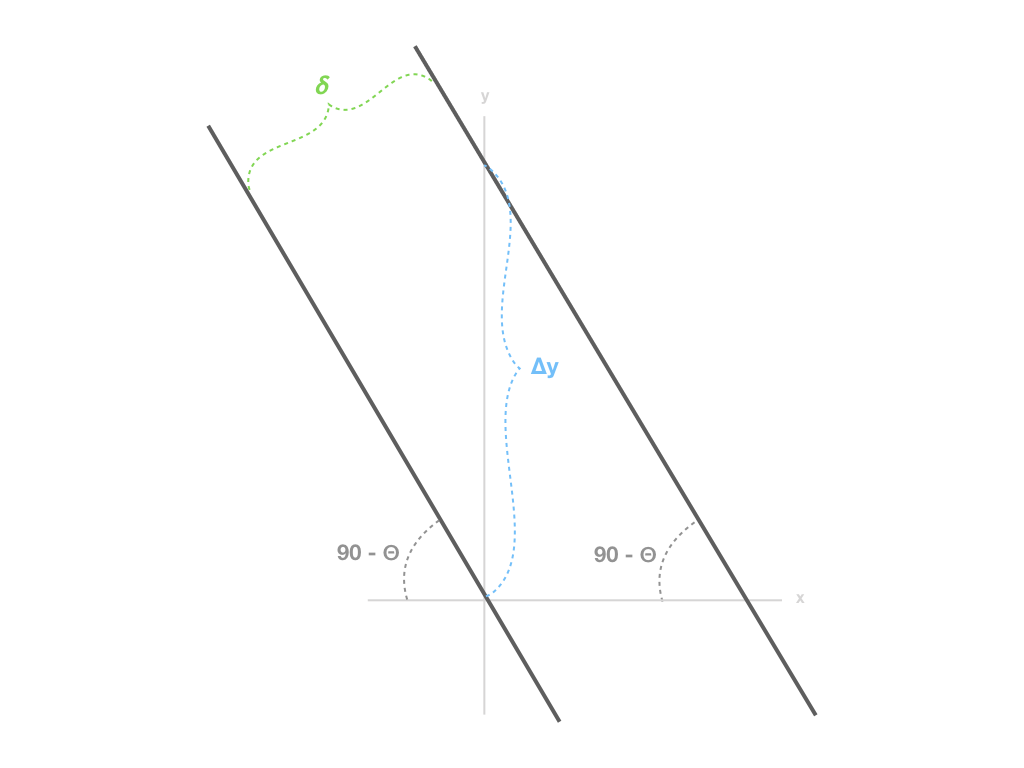
\includegraphics[width=0.9\textwidth]{figures/deltay.png}
  \caption{Parallel rays at an angle}
  \label{fig:deltab}
\end{figure}